\section{Additive Effect Sites}

This assay is designed to detect sites witth small-effect fitness contributions.
Although knockout effects of individual sites do not reach the threshold for detectability, knocking out several may.
This assay assumes a preliminary set of single-site knockouts that exclude sites with individually-detectable fitness effects from further consideration.
Then, sets of remaining sites are sampled and knocked outt together.

In the presence of small-effect sites, a classic dose-response curve will occur as sampled set size is increased.
That is, detectable fitness effects will be observed more frequently for larger knockout sets.
The shape of this dose curve will depend on both the abundance of small-effect sites and their mean effect size.
Fitting a negative binomial distribution to the curve allows these factors to estimated.
This distribution models, for coin flips with success probability $p$, the number of successive trials required to achieve $n$ successes.
If we consider resolution of sampled sites to small-effect versus true-neutral categories as a coin flip event, then the proportion of small-effect sites will correspond to $p$ and $n$, the number of required small-effect sites to reach detctability, will be inverse to the mean effect size.
Under this framming, the dose response curve corresponds to the cumulative disribution function of an underlying negative binomial distribution.

For an initial experiment exploring this approach, we generated a sammple genome with 1,000 sites, 50 of which were designated to be small-effect siters.
Effect sizes for these sites were uniformly between 0 and 0.2, relative to the detectability threshold of 1.0.
To decide dose levels for the main assay, we first sampled 250 doses spread evenly from 1 to 1,000 sites and tested for detectable fitness effects for one sample at each dose level.
We used the interval between the lowest dose with a detected fitness effect and the highest dose without a detected fitness effect as the dosing range for the main assay, choosing five dosing levels spaced evenly across this range.
For this trial, our selected dose levels were 87, 136, 186, 236, and 286 sites.
We then performed 1,000 knockouts of site sets sampled at each level.
Resulting estimates of the additive site count and mean effect size were both accurate, matching the true values of 50.0 and 0.1, respectively.

\section{Epistatic Effect Sites}

\begin{figure}
  \centering
  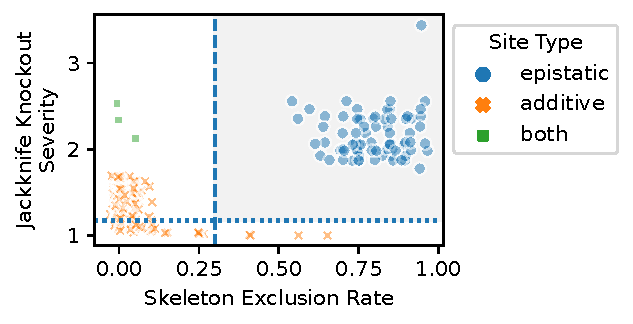
\includegraphics[width=\linewidth]{binder/teeplots/hue=site-type+style=site-type+viz=scatterplot-rect+x=skeleton-exclusion-rate+y=jackknife-knockout-severity+ext=}
  \vspace{-0.25in}
  \caption{%
    Use of knockout effect sizes and inclusion rates within ``skeletonized'' minimal viable genomes to distinguished small-effect and epistatic genome sites.
  }
  \label{fig:epistatic}
  \vspace{-0.25in}
\end{figure}


This assay is designed to detect sites that only express detectable fitness knockout effects in the presence of specific other knockouts due to redundancy or epistatic masking.
Because only one among a set of redundant sites will appear in any skeleton, the frequency with which redundant sites are excluded from skeletons should relatively high.
However, some very small effect additive sites will also be frequently excluded from skeletons.
To disambigute these scenarios, we propose an additional step: ``jackknife'' one-by-one knockouts of each site within sampled skeletons.
Jackknifed sites with detectable, butt very small magnitude fitness effects can then be identified as likely additive,  rather. than epistatic.

For an initial experiment exploring this approach, we generated a sammple genom with 4,000 sites, 200 of which were designated to be small-effect sites.
Effect sizes for these sites were uniformly between 0 and 0.7, relative to the detectability threshold of 1.0.
We additionally introduced 20 sets of 5 redundnat sites.
Fitness penalties uniformly distributed between 0.7 and 1.6 units were incurred when all sites within a set were knocked out.
We then generated 20 sample skeletons through independent strip-down procedures, knockout out sites until no more could be removed without detectable fitness effects.
After performing Jackknife knockouts of each skeleton, we plotted skeleton exclusion frequency versus mean jackknive severity for each site that appeared in any skeleton.
As shown in Figure \ref{fig:epistatic}, epistatic sites fall into the upper right quadrant.
This procedure was able to identify 80 of the true 94 epistatic sites in the sample genome.

\section{Any Effect Sites}

Any genome site with some fitness benefit should, in principle, potentially appear within a genome skeleton.
Put another way, skeletons sample randomly (although not uniformly) from genome sites with some fitness benefit.
Under this framing, the composition of genome skletons can be analogized to the content of traps used by wildlife biologists to estimate the size of animal populations.
In these scenarios, individuals tend to have lower recapture counts when membered within a large population.
Robust statistical procedures have been developed to account for biasing factors, including variation in capture probabilities among individuals (``trap shyness'') \citep{amstrup2010handbook}.
In this work, we use the Burnham-Overton procedure to estimate the total number of any-effect sites from the distribution of capture counts among sites appearing within skeleton genomes \citep{burnham1979robust}.

For an initial experiment exploring this approach, we generated sammple genomes with 10,000 sites, 395 of which were designated to be small-effect sites, 155 were designated epistatic, and 5 were both small-effect and epistatic.
Effect sizes for the small-effect sites were uniformly between 0 and 0.7, relative to the detectability threshold of 1.0.
Epistatic sites were organized into 40 4-site sets, with a fitness penalty between 0.7 and 1.6 units incurred when all sites within a set were knocked out.
We used progressive knockouts to sample 5 skeletons, with 504 distinct sites appearing in at least one skeleton.
The Burnham-Overton estimation procedure estimated 558 any-effect sites, close to the true count off 555 any-effect sites.
The 95\% confidence interval for this estimation was between 533 and 583 sites.

% Create Sample Genome
% Create a genome with 10,000 distinct sites.

% Let 4% of sites have a knockout fitness effect below detectability threshold. Effect sizes are distributed uniformly between 0 and 0.7, relative to the detectability threshold of 1.0.

% Add 40 epistatic sets, each with 4 sites. Fitness consequences of magnitudes between 0.7 and 1.6 occur when all sites within an epistatic set are knocked out.

% Overlap is allowed --- n individual sites may have both additive and epistatic effects.

% num_sites = 10000
% distn = lambda x: np.random.rand(x) * 0.7
% additive_array = create_additive_array(num_sites, 0.04, distn)
% epistasis_matrix = create_epistasis_matrix_disjoint(num_sites, 40, 4)
% genome = GenomeExplicit(
%     [
%         CalcKnockoutEffectsAdditive(additive_array),
%         CalcKnockoutEffectsEpistasis(epistasis_matrix, effect_size=(0.7, 1.6)),
%     ],
% )

% neutral      9445
% additive      395
% epistasis     155
% both            5
% Name: site type, dtype: int64

% How many functional (i.e., non-neutral) sites are there?

% num_functional_sites = (df_genome["site type"] != "neutral").sum()
% num_functional_sites
% 555
% Perform Skeletonizations
% "Skeletons" are minimal sets of genome sites that maintain wile-type fitness. Skeletons can be generated by sequentially removing sites from the genome, until no further sites can be removed without detectably reducing fitness.

% How many unique sites show up in any skeleton? (i.e., num sites with direct evidence of functionality)

% np.any(
%     (~skeletons.astype(bool)),
%     axis=0,
% ).sum()
% 504
% Estimate Number Functional Sites
% The skeletonization process can actually be interpreted as a mark-recapture experiment. Just like field researchers counting rabbits, we can estimate the total population of functional sites from the rate at which we "re-capture" specimens. (Here, "re-capture" means that a site is included in more than one skeleton.)

% Note that statistics taking into account bias in capture probability (aka "trap shyness") are necessary. This implementation uses a nonparametric jackknife estimator due to Burnham and Overton (see source code for details).

% assay_agnostic_naive(df_skeletons)
% {'num sites estimate': 558.3499999999999,
%  'num sites 95% CI': (533.2059805122569, 583.4940194877429)}
% For comparison the actual number of functional sites is

% num_functional_sites
% 555
